\documentclass[12pt]{article}
\usepackage[english]{babel}
\usepackage[letterpaper,margin=1in]{geometry}
\usepackage[parfill]{parskip}
\usepackage{graphicx}
\usepackage{mathtools}
\usepackage{amssymb}
\graphicspath{{img/}}
\usepackage{hyperref}
\frenchspacing
\author{Ariel Davis (azdavis), Jerry Yu (jerryy)}
\date{\today}
\title{15-418 Final Project Report}
\begin{document}
\maketitle

\section{Overview}

We implemented portrait mode in parallel.
Portrait mode has traditionally been done by high end DSLR camera hardware,
which the foreground of the subject is in focus and the background is blurred.
We have chosen to use a software-only image processing approach to this problem,
segmenting the image into the foreground and blurring the background.

On our largest images, we were able to achieve 150x speedup with CUDA on GPUs
and 11x speedup with OpenMP on CPUs.

\begin{figure}[!htb]
    \begin{minipage}{0.48\textwidth}
        \centering
        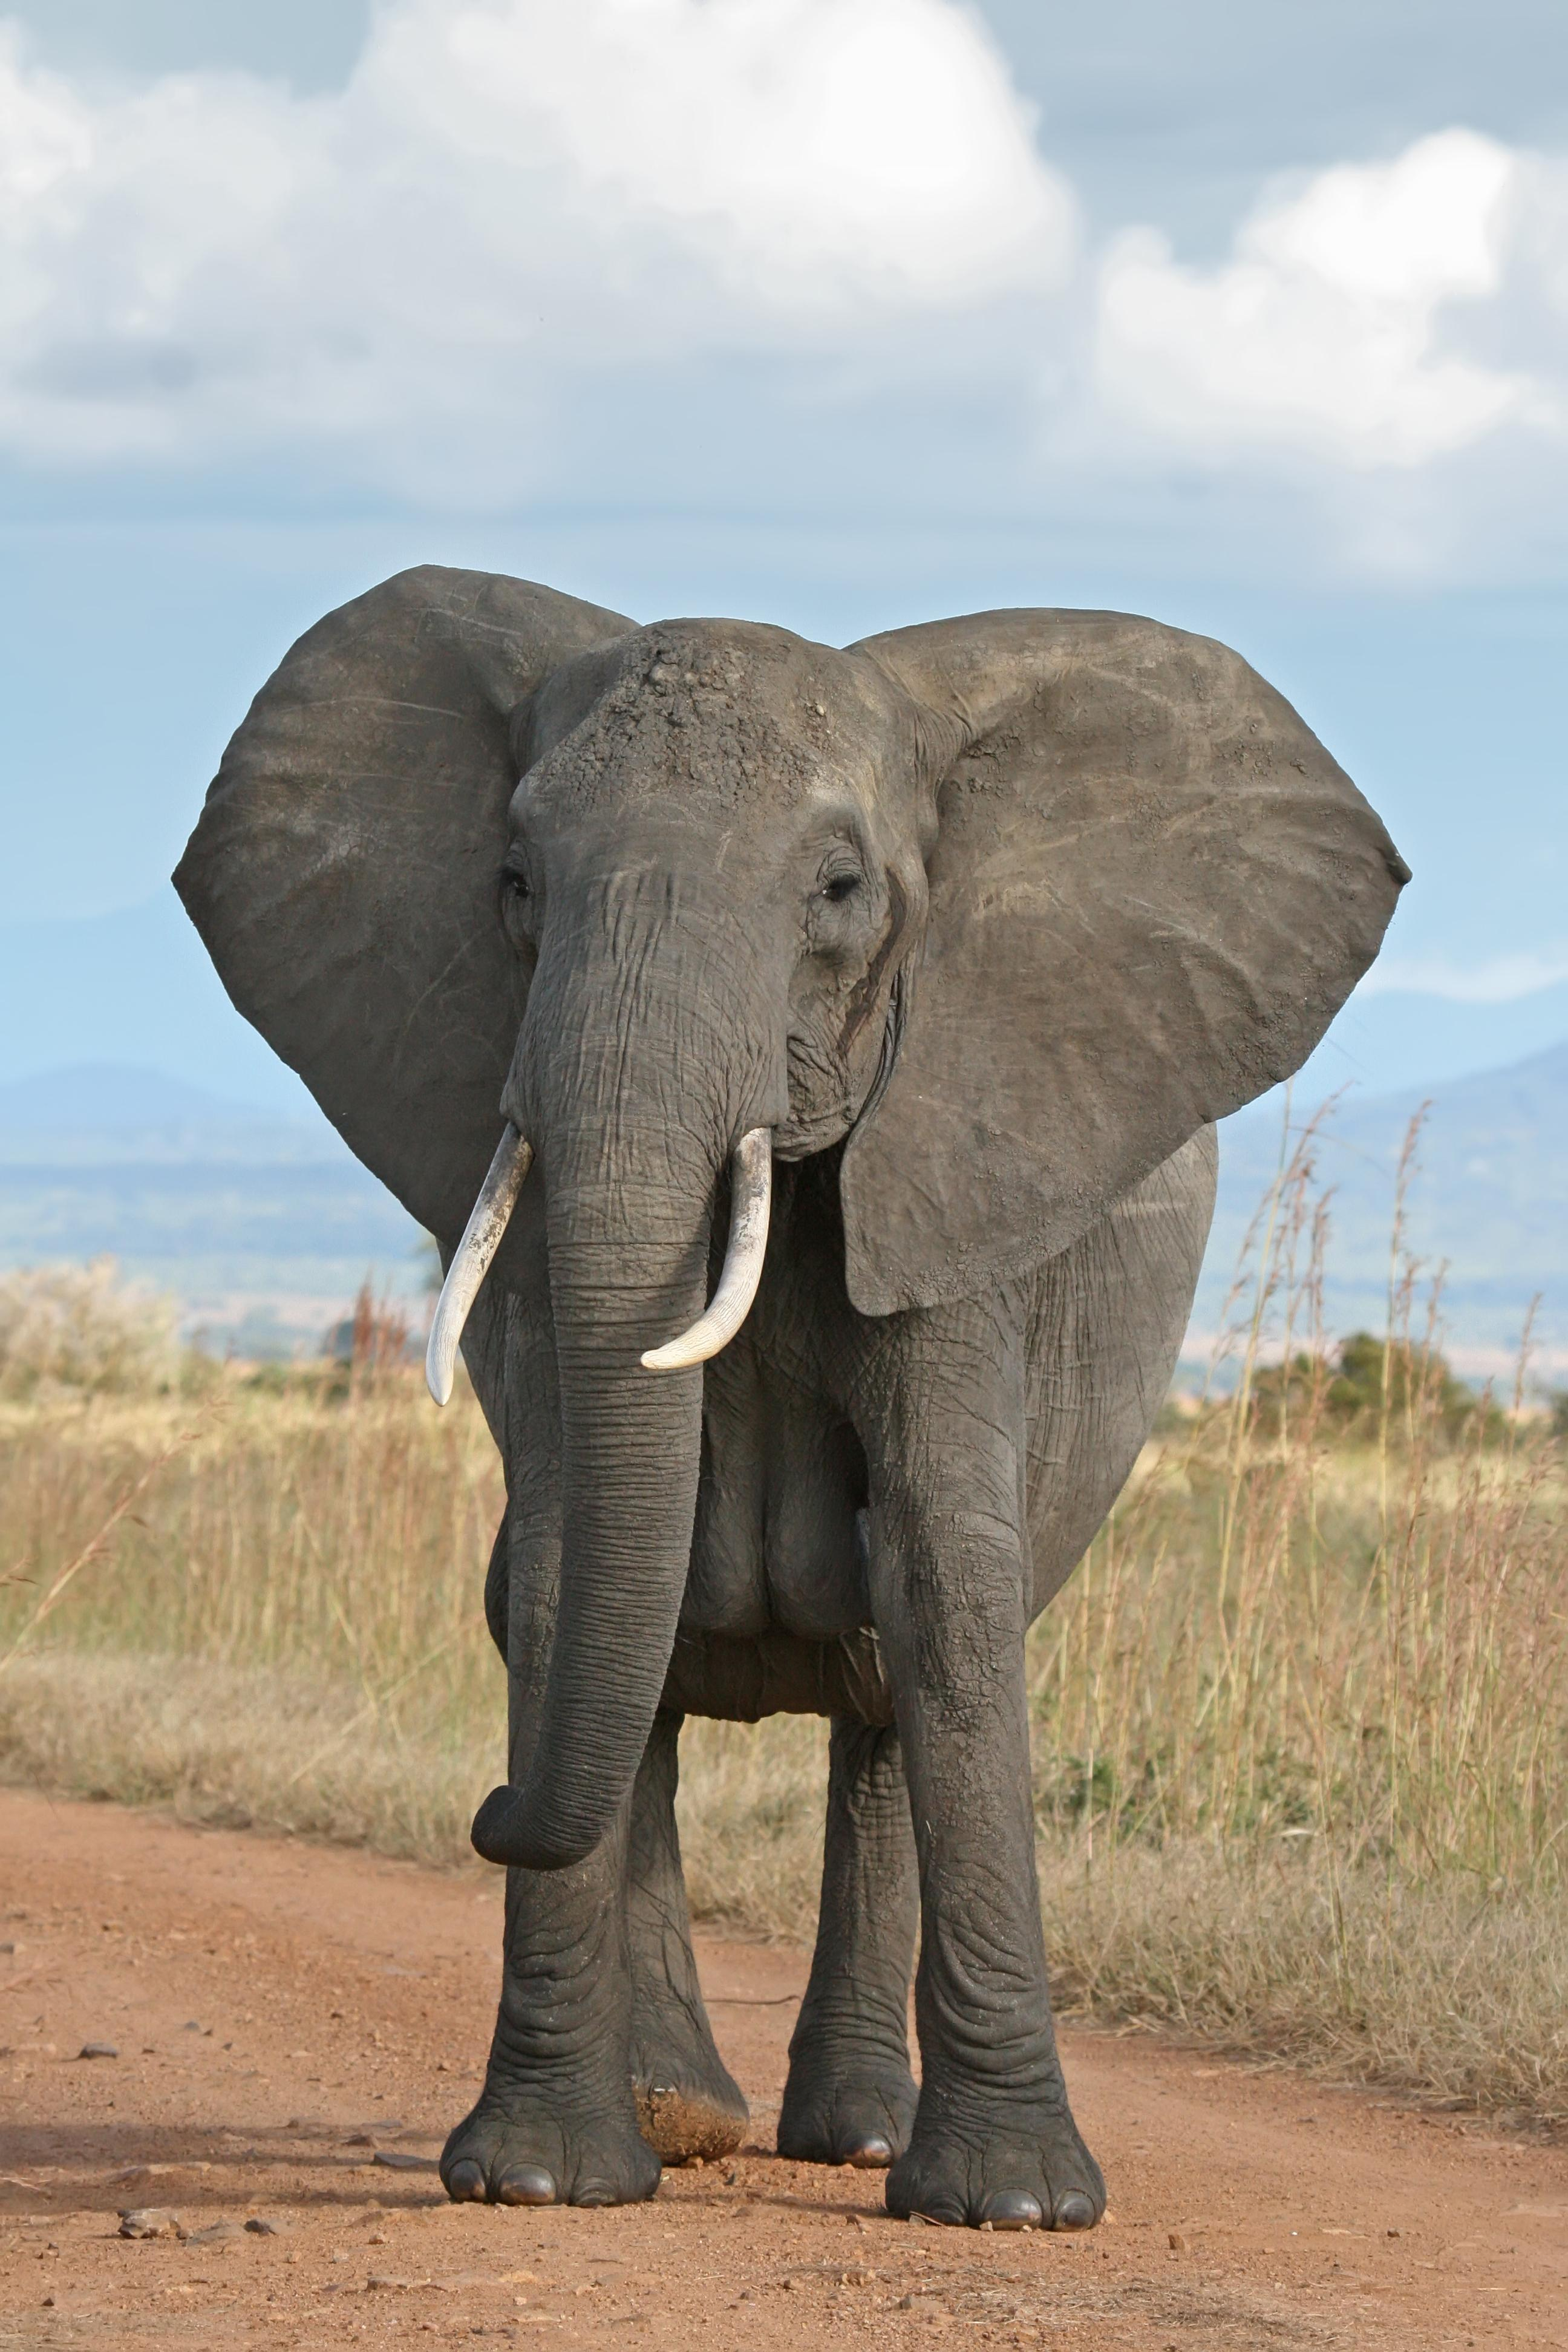
\includegraphics[width=0.9\linewidth]{large_elephant.jpg}
        \caption{Input Image}
    \end{minipage}\hfill
    \begin{minipage}{0.48\textwidth}
        \centering
        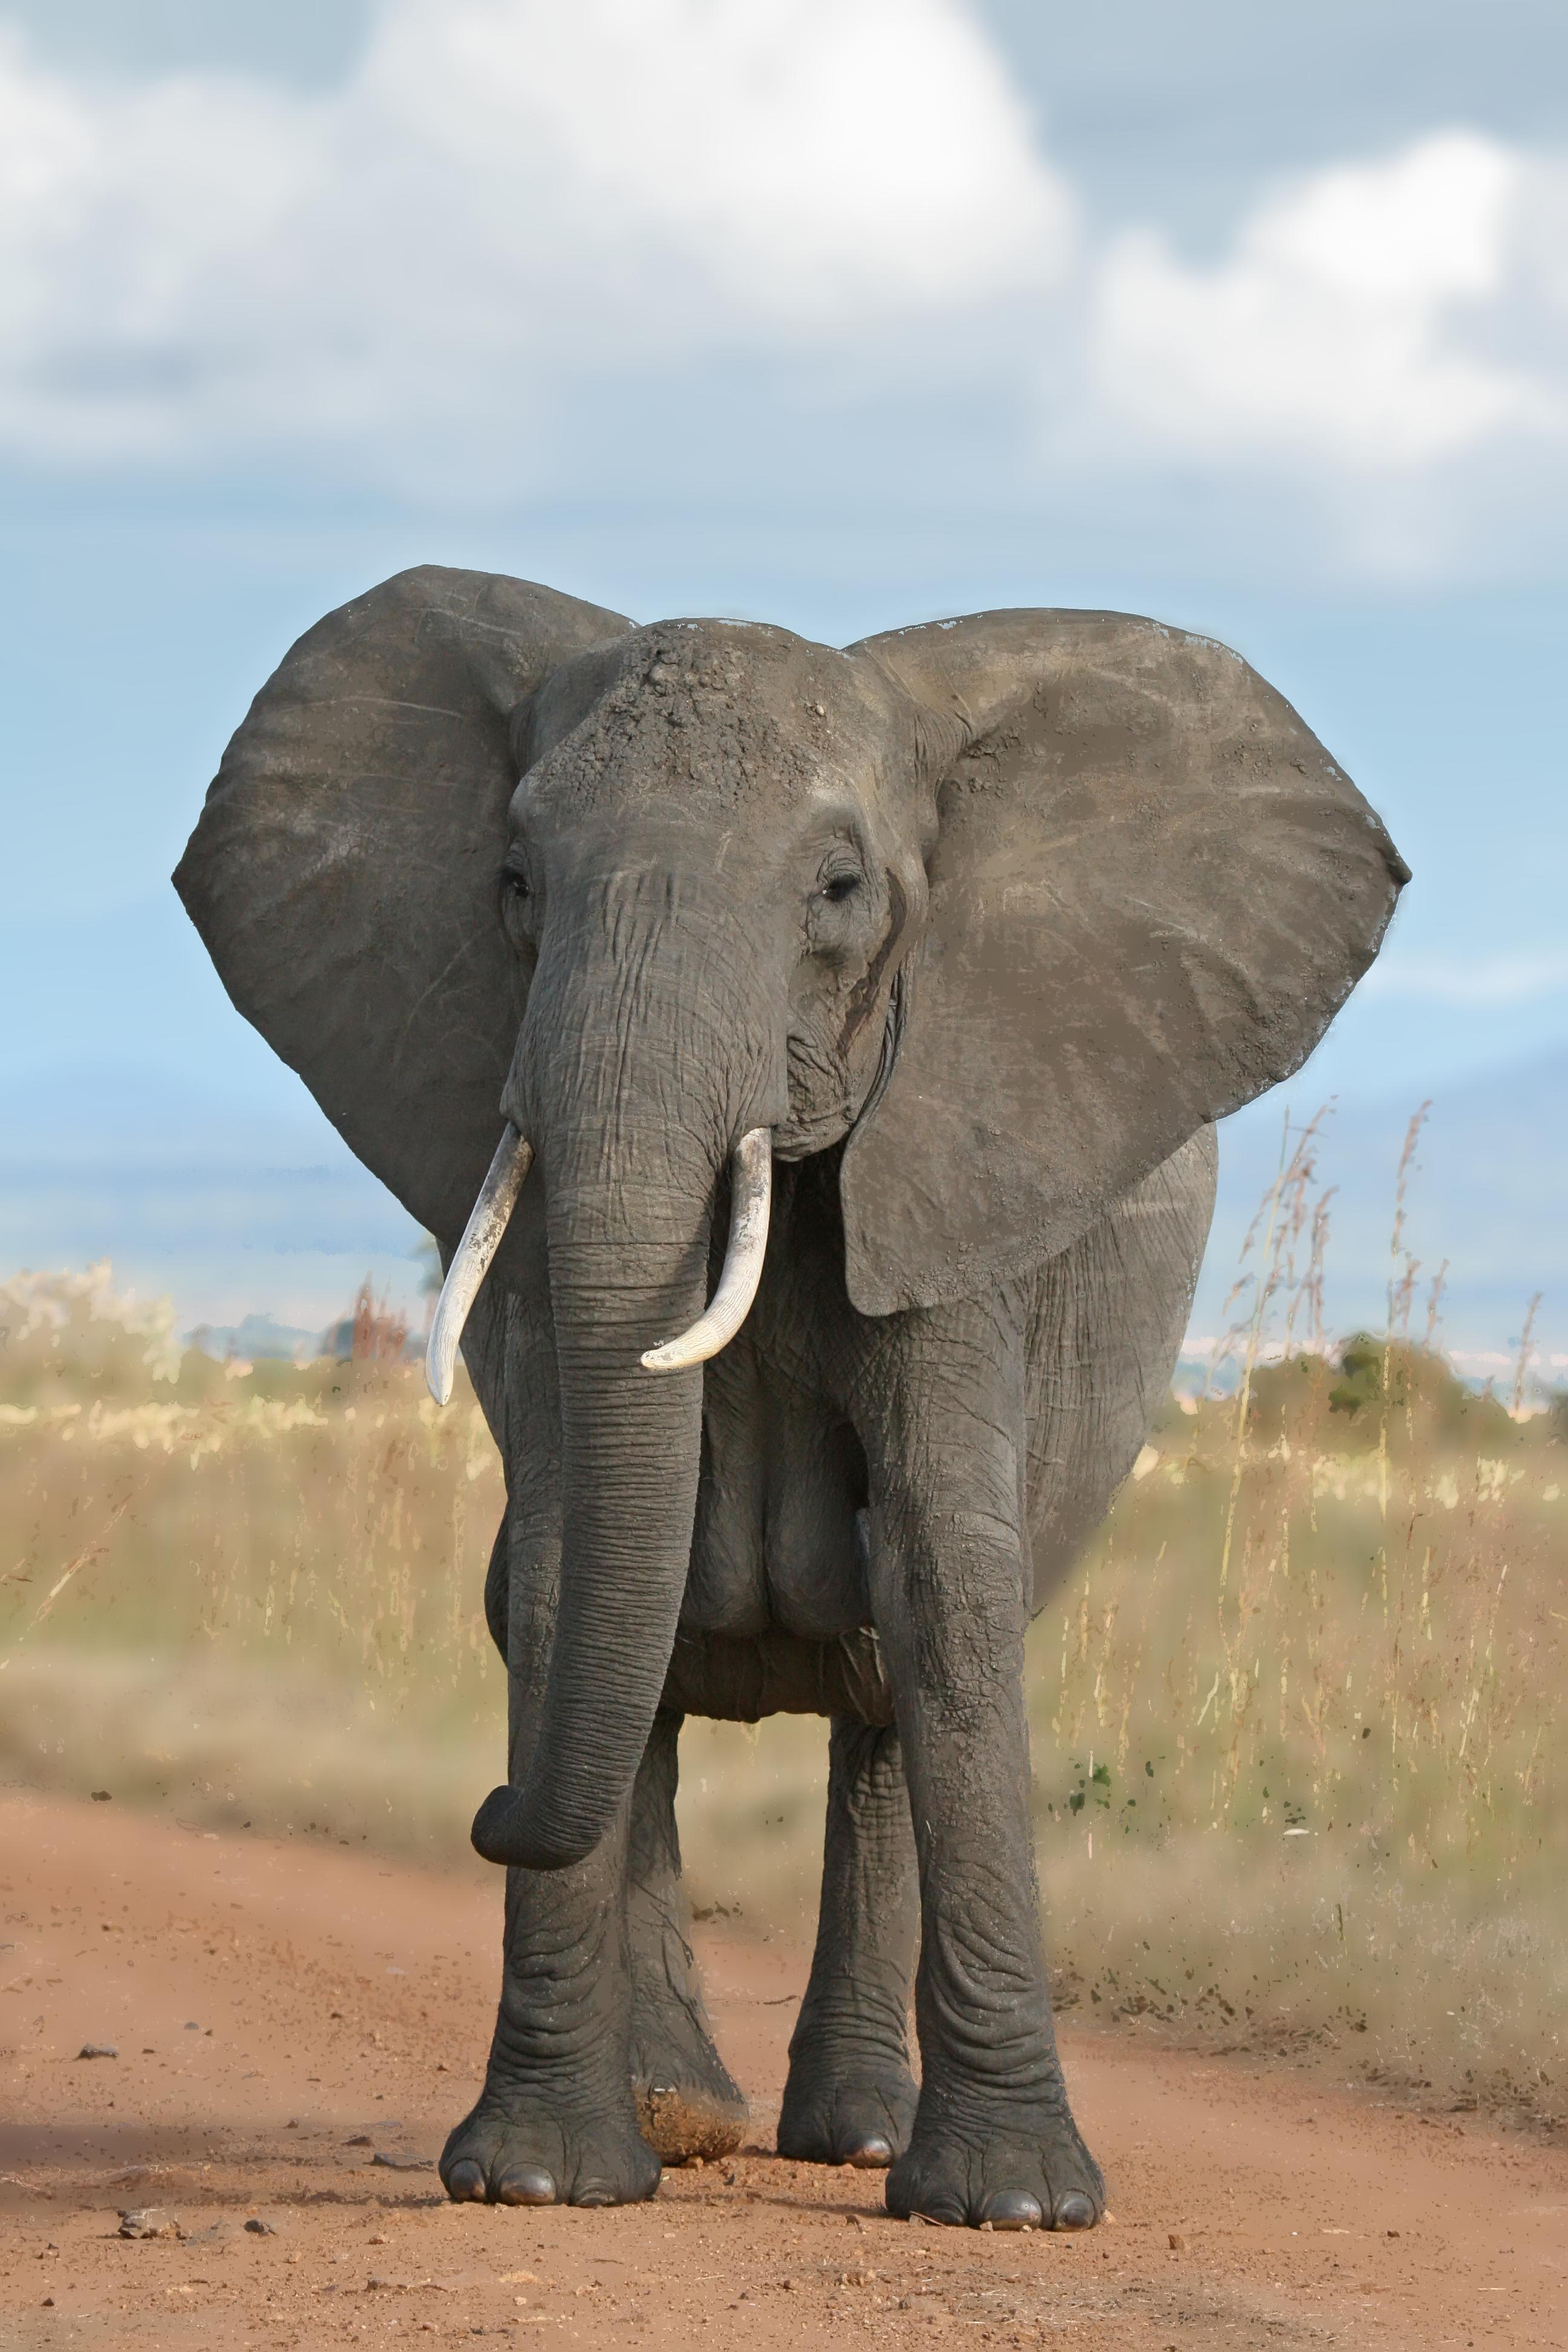
\includegraphics[width=0.9\linewidth]{large_elephant_portrait.jpg}
        \caption{Output Portrait Mode Image}
    \end{minipage}\hfill
\end{figure}

\section{Algorithm}

We used a simplified version of the grab-cut algorithm, with the idea of getting
the color distribution of the background to find the foreground.
Our algorithm takes in input image and returns the image in portrait mode.
Each image is represented as an array of pixels, with each pixel representing
a red, green, and blue value.

\begin{enumerate}
    \item
        Designiate the borders of the image as the background. Top, left, and
        right $\tfrac{1}{8}$ of image.
    \item
        Get a color distribution of the background region. Group colors together
        based on a certain threshold.
    \item
        Filter colors that make up less than 1 percent of the background area.
    \item
        Create a foreground mask by finding every pixel with a color not
        in the background color distrubution.
    \item
        For every unmasked pixel, add it to the mask if two of its neighboring
        pixels were part of the mask.
    \item
        Blur all the pixels that are not within the foreground mask. We used a
        circular filter to emulate the bokeh effect.
    \item
        For each pixel in the mask, add the original pixel of the image into
        the blurred version of the image.
\end{enumerate}

The blur is the most computationally intensive part of the algorithm. Each pixel
of the blurred image needs to compute the average RGB values for a circle
of pixels around it. However, the blur is data parallel, as each pixel is
independent.

However, each step of the algorithm hsa to be finished before the next step.
This requires synchronization after each step.



\begin{figure}[!htb]
    \begin{minipage}{0.48\textwidth}
        \centering
        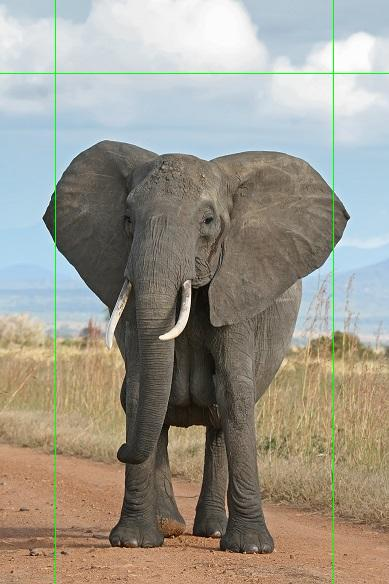
\includegraphics[width=0.5\linewidth]{border.jpg}
        \caption{Background Region (Step 1)}
    \end{minipage}\hfill
    \begin{minipage}{0.48\textwidth}
        \centering
        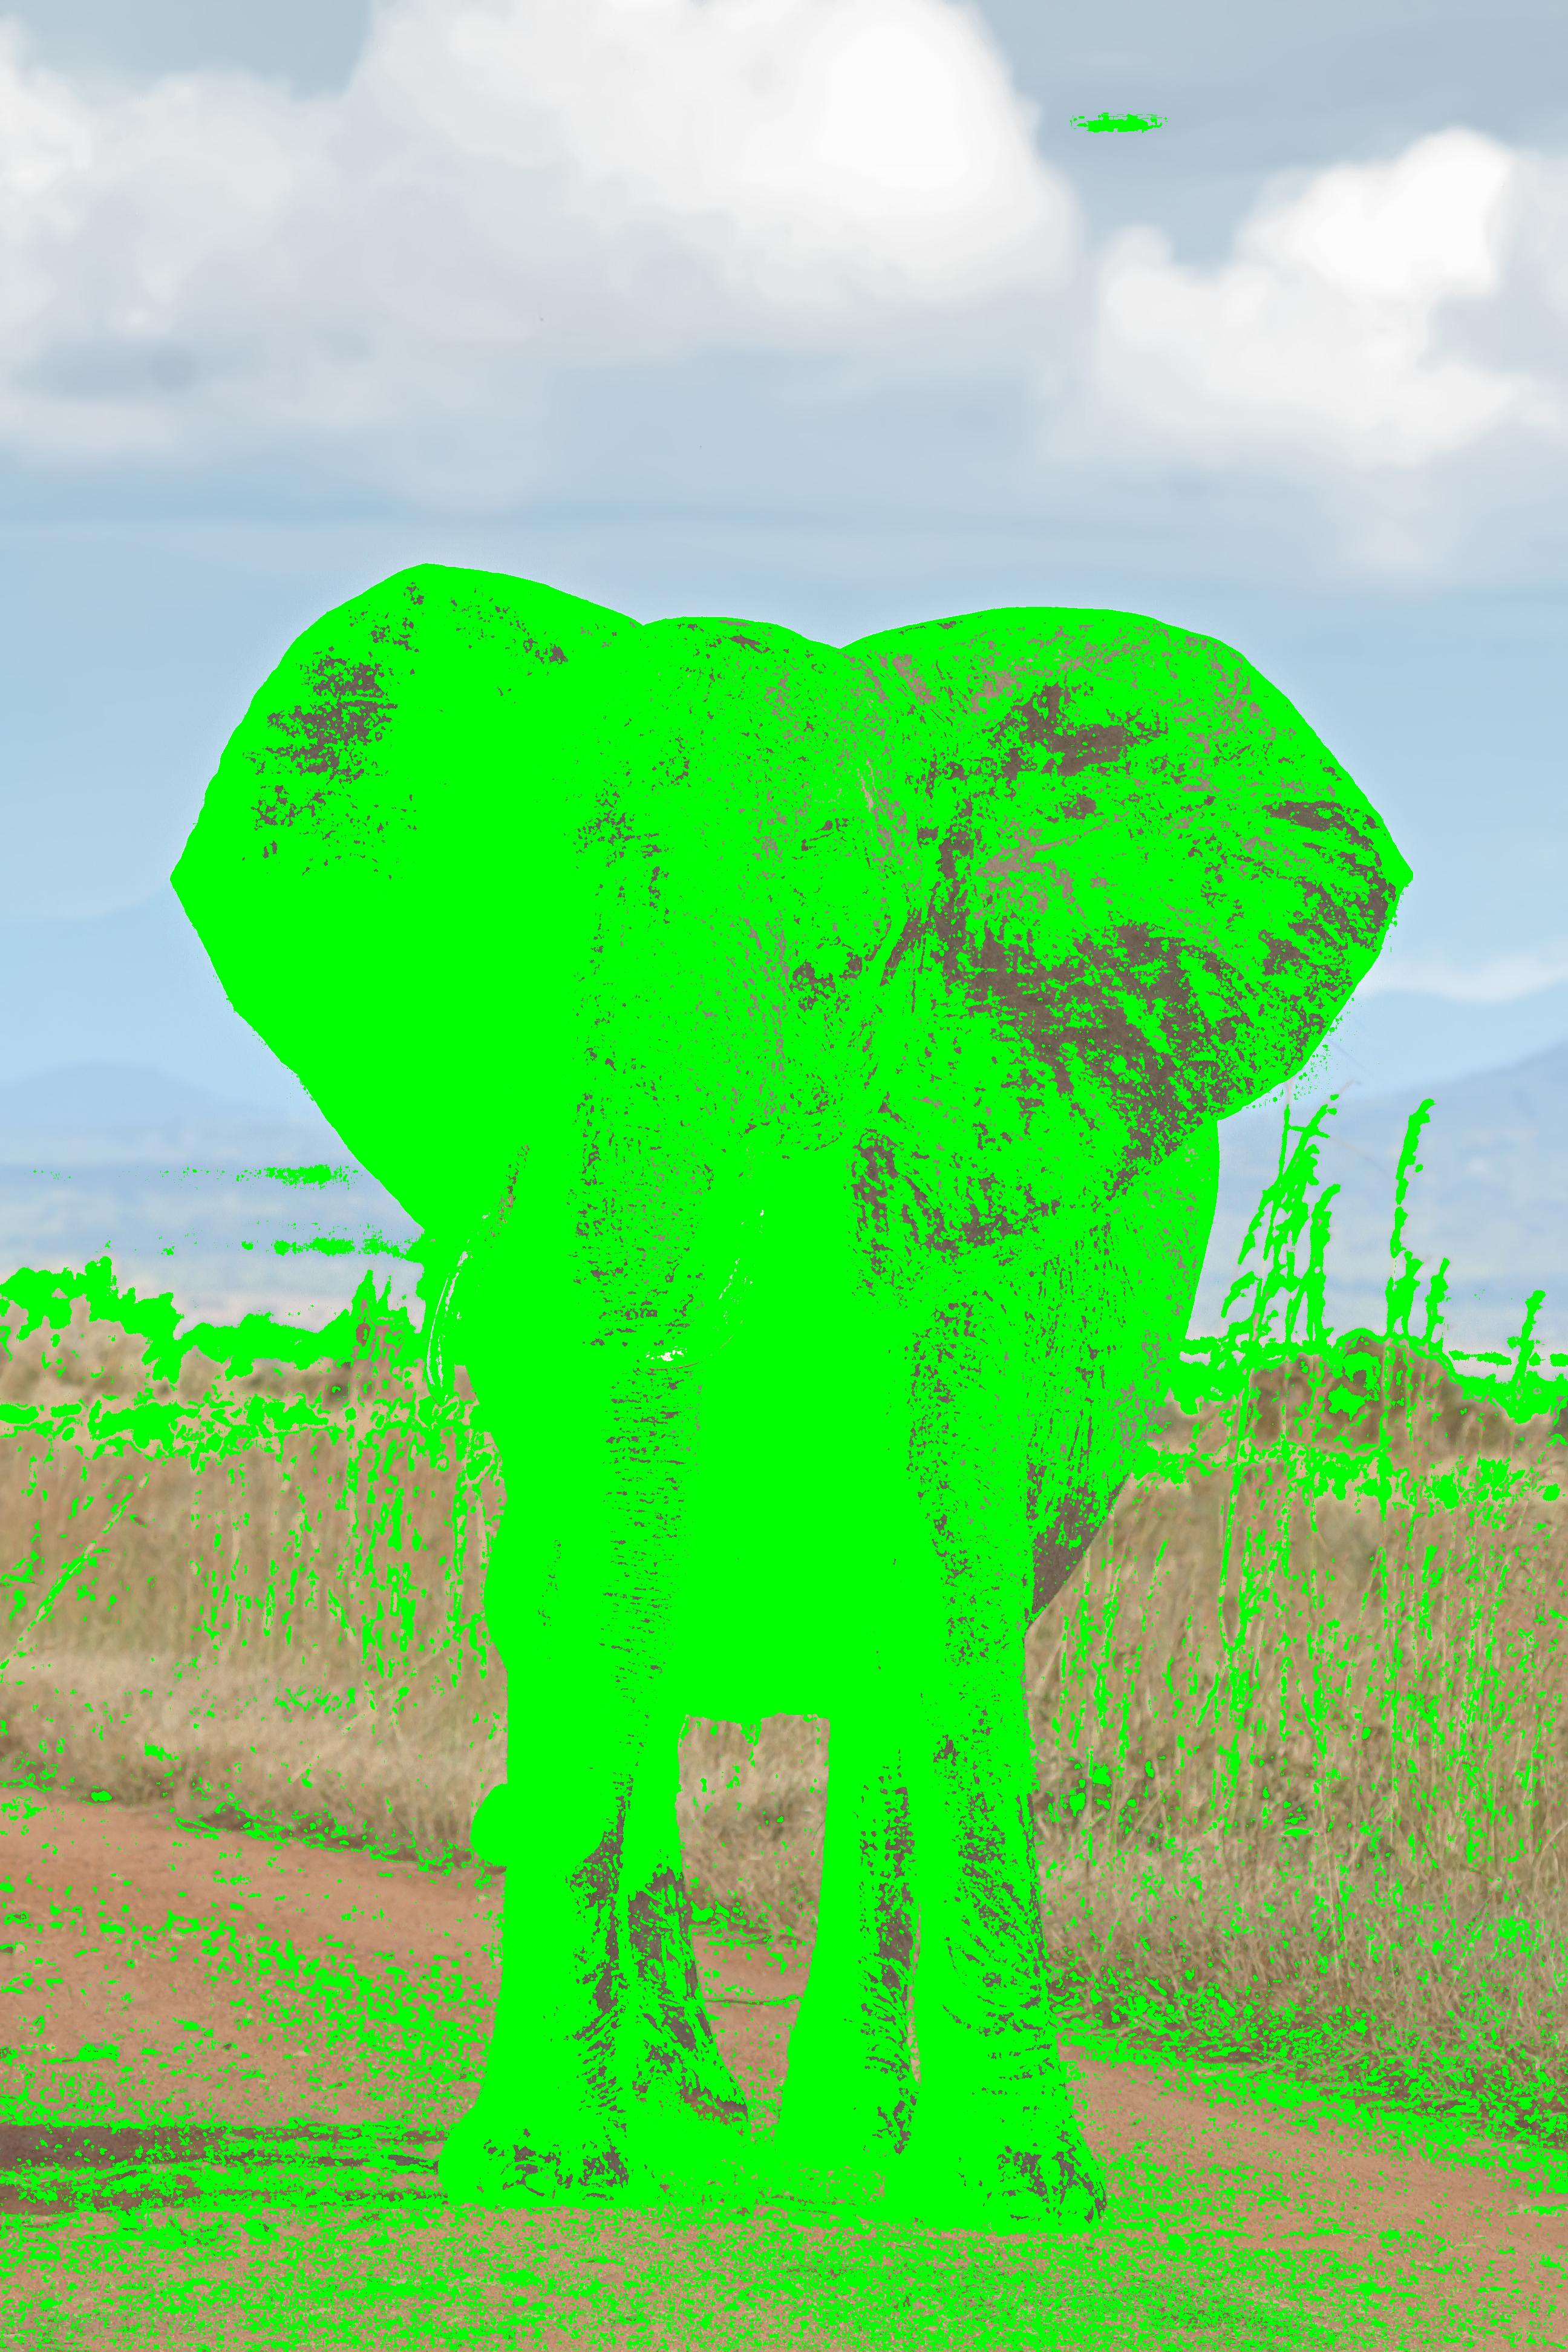
\includegraphics[width=0.5\linewidth]{mask.jpg}
        \caption{Foreground Mask (Step 5)}
    \end{minipage}\hfill
\end{figure}

\begin{tabular}{l|l|l|l|l|l}
    Image (size in px) & C & OMP & OMP Speedup & Cuda & Cuda Speedup \\
    \hline
    Large Elephant 2594x3888 & 111.52s & 9.972s & 11.19x & 0.748s & 150.43x \\
\end{tabular}

\begin{tabular}{l|l|l|l|l|l}
    Task & C & OMP & OMP Speedup & CUDA & CUDA Speedup\\
    \hline
    Load Image & 0.0123s & 0.0159s & - & 0.0077s & -\\
    CUDA Move Memory & - & - & - & 0.1815s & -\\
    Generate Mask & 0.1500s & 0.0608s & 2.44x & 0.0027s & 55.56x\\
    Blur & 111.6798s & 9.507s & 11.75x & 0.1949s & 573.01x \\
    Write Image & 0.3258s & 0.3596s & - & 0.3186 & -
\end{tabular}

\end{document}
